\section{黎曼曲面的定义}
\sourcepage{1}
本节定义黎曼曲面、其上的全纯函数和亚纯函数，以及黎曼曲面之间的全纯映射。

黎曼曲面是带有某种附加结构的二维流形，我们即将定义这种结构。众所周知，$n$维流形是一个Hausdorff拓扑空间$X$，其中每一点$a\in X$都有一个与$\R^n$中某个开子集同胚的开邻域。
\sourcepage{2}
\entry{1.1}{定义}
设$X$是二维流形。$X$上的一个\textbf{复坐标卡}（complex chart）是从开子集$U\subset X$到开子集$V\subset\C$的一个同胚$\varphi:U\to V$。称两个复坐标卡$\varphi_i:U_i\to V_i$（$i=1,2$）\textbf{全纯相容}（holomorphically compatible），如果映射
\[
\varphi_2\circ\varphi_1^{-1}:\varphi_1(U_1\cap U_2)\longrightarrow\varphi_2(U_1\cap U_2)
\]
是双全纯的（见图1）。
\begin{center}\begin{minipage}{\linewidth}\centering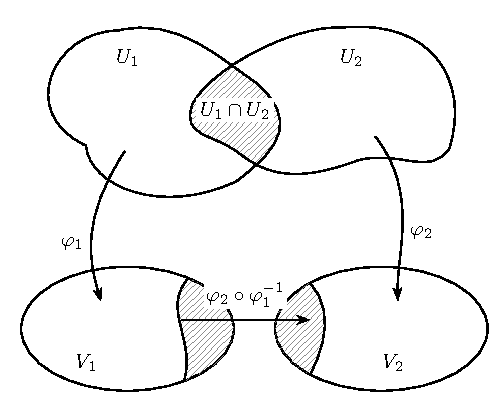
\includegraphics[width=.62\textwidth]{figures/fig01-tikz.pdf}\\图1\end{minipage}\end{center}
$X$上的一个\textbf{复图册}（complex atlas）是由彼此全纯相容的坐标卡组成的族
$\mathfrak A=\{\varphi_i:U_i\to V_i,\ i\in I\}$，并且它们覆盖$X$，即$\bigcup_{i\in I}U_i=X$。

称$X$上的两个复图册$\mathfrak A$和$\mathfrak A'$\textbf{解析等价}（analytically equivalent），如果$\mathfrak A$中的每一张坐标卡都与$\mathfrak A'$中的每一张坐标卡全纯相容。

\entry{1.2}{注记}
(a) 若$\varphi:U\to V$是复坐标卡，$U_1$是$U$中的开集，且$V_1:=\varphi(U_1)$，则$\varphi|_{U_1}:U_1\to V_1$是一张与$\varphi:U\to V$全纯相容的坐标卡。

(b) 由于双全纯映射的复合仍是双全纯映射，容易看出，复图册的解析等价关系是一个等价关系。

\entry{1.3}{定义}
二维流形$X$上的一个\textbf{复结构}（complex structure），是$X$上解析等价图册的一个等价类。

因此，选定一个复图册便可给出$X$上的一个复结构。$X$上的每个复结构$\Sigma$都包含唯一的极大图册$\mathfrak A^*$。若$\mathfrak A$是$\Sigma$中任一图册，则$\mathfrak A^*$恰由$X$上所有与$\mathfrak A$中的每张坐标卡全纯相容的复坐标卡组成。
\sourcepage{3}
\entry{1.4}{定义}
\textbf{黎曼曲面}（Riemann surface）是一个二元组$(X,\Sigma)$，其中$X$是连通二维流形，$\Sigma$是$X$上的复结构。

只要所指的复结构$\Sigma$明确，通常就写$X$而不写$(X,\Sigma)$。有时也写$(X,\mathfrak A)$，其中$\mathfrak A$是$\Sigma$的一个代表。

\textbf{约定。}若$X$是黎曼曲面，今后所说的$X$上的坐标卡，总是指属于$X$的复结构的极大图册的复坐标卡。

\textbf{注记。}局部地看，黎曼曲面$X$就是复平面中的一个开集。事实上，若$\varphi:U\to V\subset\C$是一张坐标卡，则$\varphi$把开集$U\subset X$双射到$V$。然而，$X$的任一给定点都属于许多不同的坐标卡，其中没有哪一张比其他坐标卡更特殊。因此，平面复分析中的概念，只有在双全纯映射下保持不变时，才能移植到黎曼曲面上；换言之，这些概念不能依赖某张特定坐标卡的选择。

\entry{1.5}{黎曼曲面的例子}
(a) \textbf{复平面$\C$。}它的复结构由只含恒等映射$\C\to\C$这一张坐标卡的图册定义。

(b) \textbf{区域。}设$X$是黎曼曲面，$Y\subset X$是一个区域，即连通开子集。则$Y$上存在自然的复结构，使其成为黎曼曲面：取$X$上所有满足$U\subset Y$的复坐标卡$\varphi:U\to V$作为它的图册。特别地，每个区域$Y\subset\C$都是黎曼曲面。

(c) \textbf{黎曼球面$\PP^1$。}令$\PP^1:=\C\cup\{\infty\}$，其中$\infty$是不属于$\C$的一个符号。在$\PP^1$上引入如下拓扑：开集包括$\C$中通常的开集$V$，以及形如$V\cup\{\infty\}$的集合，其中$V\subset\C$是某个紧集$K\subset\C$的补集。赋予这一拓扑后，$\PP^1$是紧Hausdorff拓扑空间，与二维球面$S^2$同胚。令
\[
U_1:=\PP^1\setminus\{\infty\}=\C,\qquad U_2:=\PP^1\setminus\{0\}=\C^*\cup\{\infty\}.
\]
如下定义映射$\varphi_i:U_i\to\C$（$i=1,2$）：$\varphi_1$是恒等映射，而
\[
\varphi_2(z):=\begin{cases}1/z,&z\in\C^*,\\0,&z=\infty.\end{cases}
\]
显然，这两个映射都是同胚，所以$\PP^1$是二维流形。又因$U_1,U_2$连通且交集非空，$\PP^1$也连通。
\sourcepage{4}
现在，由坐标卡$\varphi_i:U_i\to\C$（$i=1,2$）组成的图册定义$\PP^1$上的复结构。须证明这两张坐标卡全纯相容。但$\varphi_1(U_1\cap U_2)=\varphi_2(U_1\cap U_2)=\C^*$，且
\[
\varphi_2\circ\varphi_1^{-1}:\C^*\to\C^*,\qquad z\mapsto1/z
\]
是双全纯映射。

\textbf{注记。}记号$\PP^1$源于这样一个事实：可以把$\PP^1$看成复数域上的一维射影空间。

(d) \textbf{环面。}设$\omega_1,\omega_2\in\C$在$\R$上线性无关。定义
\[
\Gamma:=\Z\omega_1+\Z\omega_2=\{n\omega_1+m\omega_2:n,m\in\Z\}.
\]
称$\Gamma$为由$\omega_1,\omega_2$张成的\textbf{格}（lattice）（图2）。若$z-z'\in\Gamma$，则称复数$z,z'\in\C$模$\Gamma$等价。所有等价类构成的集合记为$\C/\Gamma$。令$\pi:\C\to\C/\Gamma$为典范投影，即把每一点$z\in\C$映到它模$\Gamma$的等价类的映射。
\begin{center}\begin{minipage}{\linewidth}\centering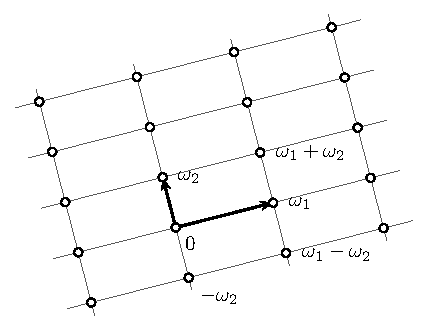
\includegraphics[width=.52\textwidth]{figures/fig02-tikz.pdf}\\图2\end{minipage}\end{center}
在$\C/\Gamma$上引入如下拓扑（商拓扑）：子集$U\subset\C/\Gamma$是开集，当且仅当$\pi^{-1}(U)\subset\C$是开集。赋予这一拓扑后，$\C/\Gamma$是Hausdorff拓扑空间，商映射$\pi:\C\to\C/\Gamma$连续。由于$\C$连通，$\C/\Gamma$也连通。此外，$\C/\Gamma$是紧的，因为紧平行四边形
\[
P:=\{\lambda\omega_1+\mu\omega_2:\lambda,\mu\in[0,1]\}
\]
在$\pi$下的像覆盖$\C/\Gamma$。映射$\pi$是开映射，即每个开集$V\subset\C$的像都是开集。为说明这一点，只须证明$\widetilde V:=\pi^{-1}(\pi(V))$是开集。但
\[
\widetilde V=\bigcup_{\omega\in\Gamma}(\omega+V).
\]
每个集合$\omega+V$都是开集，所以$\widetilde V$也是开集。
\sourcepage{5}
$\C/\Gamma$上的复结构如下定义。设$V\subset\C$是开集，且$V$中任意两点都不模$\Gamma$等价。则$U:=\pi(V)$是开集，$\pi|_V:V\to U$是同胚。它的逆映射$\varphi:U\to V$是$\C/\Gamma$上的一张复坐标卡。令$\mathfrak A$为所有以此方式得到的坐标卡所成的集合。须证明$\mathfrak A$中的任意两张坐标卡$\varphi_i:U_i\to V_i$（$i=1,2$）全纯相容。考虑映射
\[
\psi:=\varphi_2\circ\varphi_1^{-1}:\varphi_1(U_1\cap U_2)\to\varphi_2(U_1\cap U_2).
\]
对每个$z\in\varphi_1(U_1\cap U_2)$，有$\pi(\psi(z))=\varphi_1^{-1}(z)=\pi(z)$，所以$\psi(z)-z\in\Gamma$。由于$\Gamma$离散且$\psi$连续，$\psi(z)-z$在$\varphi_1(U_1\cap U_2)$的每个连通分支上都是常数。因此$\psi$全纯，同理$\psi^{-1}$也全纯。

现在赋予$\C/\Gamma$由复图册$\mathfrak A$定义的复结构。

\textbf{注记。}设$S^1=\{z\in\C:|z|=1\}$为单位圆周。把$\C/\Gamma$中由$\lambda\omega_1+\mu\omega_2$（$\lambda,\mu\in\R$）代表的点映到
\[
(e^{2\pi i\lambda},e^{2\pi i\mu})\in S^1\times S^1
\]
的映射，是$\C/\Gamma$到环面$S^1\times S^1$的同胚。

\entry{1.6}{定义}
设$X$是黎曼曲面，$Y\subset X$是开子集。称函数$f:Y\to\C$\textbf{全纯}（holomorphic），如果对$X$上的每张坐标卡$\psi:U\to V$，函数
\[
f\circ\psi^{-1}:\psi(U\cap Y)\to\C
\]
在开集$\psi(U\cap Y)\subset\C$上按通常意义全纯。$Y$上全体全纯函数构成的集合记为$\OO(Y)$。

\entry{1.7}{注记}
(a) 全纯函数的和与积仍是全纯函数，常值函数也全纯。因此$\OO(Y)$是一个$\C$代数。

(b) 当然，不必对$X$上极大图册中的所有坐标卡验证定义中的条件，只须对覆盖$Y$的任意一族坐标卡验证即可。此时其他坐标卡也自动满足这一条件。

(c) $X$上的每张坐标卡$\psi:U\to V$尤其是$U$上的一个复值函数，显然它全纯。也称$\psi$为\textbf{局部坐标}（local coordinate）或\textbf{局部一致化参数}（uniformizing parameter），并称$(U,\psi)$为任一点$a\in U$的一个\textbf{坐标邻域}（coordinate neighborhood）。在这种语境下，一般用字母$z$代替$\psi$。

\entry{1.8}{定理（Riemann可去奇点定理）}
设$U$是黎曼曲面中的开子集，$a\in U$。若函数$f\in\OO(U\setminus\{a\})$在$a$的某个邻域内有界，则$f$可唯一延拓为函数$\widetilde f\in\OO(U)$。
\sourcepage{6}
这一结果直接由复平面中的Riemann可去奇点定理得到。

现在定义黎曼曲面之间的全纯映射。

\entry{1.9}{定义}
设$X,Y$是黎曼曲面。称连续映射$f:X\to Y$\textbf{全纯}，如果对$X$上的每张坐标卡$\psi_1:U_1\to V_1$以及$Y$上的每张坐标卡$\psi_2:U_2\to V_2$，只要$f(U_1)\subset U_2$，映射
\[
\psi_2\circ f\circ\psi_1^{-1}:V_1\to V_2
\]
就按通常意义全纯。

称映射$f:X\to Y$\textbf{双全纯}（biholomorphic），如果它是双射，且$f:X\to Y$与$f^{-1}:Y\to X$都全纯。称两个黎曼曲面$X,Y$\textbf{同构}（isomorphic），如果存在双全纯映射$f:X\to Y$。

\entry{1.10}{注记}
(a) 在$Y=\C$这一特殊情形，全纯映射$f:X\to\C$显然就是全纯函数。

(b) 若$X,Y,Z$是黎曼曲面，$f:X\to Y$与$g:Y\to Z$是全纯映射，则复合$g\circ f:X\to Z$也全纯。

(c) 两个黎曼曲面之间的连续映射$f:X\to Y$全纯，当且仅当对每个开集$V\subset Y$和每个全纯函数$\psi\in\OO(V)$，“拉回”函数$\psi\circ f:f^{-1}(V)\to\C$都属于$\OO(f^{-1}(V))$。这直接由定义及注记(1.7.c)、(1.10.b)得到。

这样，全纯映射$f:X\to Y$便诱导映射
\[
f^*:\OO(V)\to\OO(f^{-1}(V)),\qquad f^*(\psi)=\psi\circ f.
\]
容易验证$f^*$是环同态。若$g:Y\to Z$是另一个全纯映射，$W$在$Z$中开，$V:=g^{-1}(W)$且$U:=f^{-1}(V)$，则$(g\circ f)^*:\OO(W)\to\OO(U)$是映射$g^*:\OO(W)\to\OO(V)$与$f^*:\OO(V)\to\OO(U)$的复合，即$(g\circ f)^*=f^*\circ g^*$。

\entry{1.11}{定理（恒等定理）}
设$X,Y$是黎曼曲面，$f_1,f_2:X\to Y$是两个全纯映射。若它们在一个具有聚点$a\in X$的集合$A\subset X$上相等，则$f_1,f_2$恒等。

\begin{proof}
令$G$为所有具有开邻域$W$使$f_1|_W=f_2|_W$的点$x\in X$所成的集合。按定义，$G$是开集。我们断言$G$也是闭集。事实上，设$b$是$G$的边界点。由$f_1,f_2$连续，有$f_1(b)=f_2(b)$。选取$X$上的坐标卡$\varphi:U\to V$和$Y$上的坐标卡$\psi:U'\to V'$，使$b\in U$且$f_i(U)\subset U'$。还可假设$U$连通。映射
\[
g_i:=\psi\circ f_i\circ\varphi^{-1}:V\to V'\subset\C
\]
\sourcepage{7}
全纯。由于$U\cap G\ne\varnothing$，由$\C$中区域上全纯函数的恒等定理可知$g_1,g_2$恒等，故$f_1|_U=f_2|_U$。于是$b\in G$，从而$G$为闭集。由于$X$连通，或者$G=\varnothing$，或者$G=X$。但再次使用平面上的恒等定理可得$a\in G$，所以第一种情况不可能。因此$f_1,f_2$在整个$X$上相等。
\end{proof}

\entry{1.12}{定义}
设$X$是黎曼曲面，$Y$是$X$的开子集。$Y$上的一个\textbf{亚纯函数}（meromorphic function）是一个全纯函数$f:Y'\to\C$，其中$Y'\subset Y$是开子集，且满足：
\begin{enumerate}[label=(\roman*)]
\item $Y\setminus Y'$只含孤立点；
\item 对每个$p\in Y\setminus Y'$，有$\displaystyle\lim_{x\to p}|f(x)|=\infty$。
\end{enumerate}
称$Y\setminus Y'$中的点为$f$的\textbf{极点}（pole）。$Y$上全体亚纯函数构成的集合记为$\MM(Y)$。

\entry{1.13}{注记}
(a) 设$(U,z)$是$f$的极点$p$的一个坐标邻域，且$z(p)=0$。则在$p$的某个邻域内，$f$可展开为Laurent级数
\[
f=\sum_{\nu=-k}^{\infty}c_\nu z^\nu,\qquad c_{-k}\ne0.
\]
(b) $\MM(Y)$具有自然的$\C$代数结构。首先，两个亚纯函数$f,g\in\MM(Y)$的和与积，在$f,g$都全纯的点处是全纯函数。然后利用Riemann可去奇点定理，将$f+g$（相应地，$fg$）越过所有可去奇点作全纯延拓。

\entry{1.14}{例}
设$n\ge1$，令
\[
F(z)=z^n+c_1z^{n-1}+\cdots+c_n
\]
为一个多项式。则$F$定义了全纯映射$F:\C\to\C$。若把$\C$视为$\PP^1$的子集，则$\lim_{z\to\infty}|F(z)|=\infty$。因此$F\in\MM(\PP^1)$。

现在把亚纯函数解释为到黎曼球面的全纯映射。

\entry{1.15}{定理}
设$X$是黎曼曲面，$f\in\MM(X)$。对$f$的每个极点$p$，定义$f(p):=\infty$。则$f:X\to\PP^1$是全纯映射。反过来，若$f:X\to\PP^1$是全纯映射，则$f$或者恒等于$\infty$，或者$f^{-1}(\infty)$只含孤立点，且$f:X\setminus f^{-1}(\infty)\to\C$是$X$上的亚纯函数。
\sourcepage{8}
今后将亚纯函数$f\in\MM(X)$与对应的全纯映射$f:X\to\PP^1$视为同一对象。
\begin{proof}
(a) 设$f\in\MM(X)$，$P$为$f$的极点集。则$f$诱导映射$f:X\to\PP^1$，它显然连续。设$\varphi:U\to V$和$\psi:U'\to V'$分别是$X$和$\PP^1$上的坐标卡，且$f(U)\subset U'$。须证明
\[
g:=\psi\circ f\circ\varphi^{-1}:V\to V'
\]
全纯。由于$f$在$X\setminus P$上全纯，$g$在$V\setminus\varphi(P)$上全纯。故由Riemann可去奇点定理，$g$在整个$V$上全纯。

(b) 逆命题由恒等定理(1.11)得到。
\end{proof}

\entry{1.16}{注记}
由(1.11)及(1.15)可知，恒等定理对黎曼曲面上的亚纯函数也成立。因此，任一不恒为零的函数$f\in\MM(X)$只有孤立零点。这表明$\MM(X)$是一个域。

\subsection*{习题（第1节）}
\entry{1.1}{}
(a) \textbf{$\R^n$的单点紧化。}设$n\ge1$，令$\infty$为不属于$\R^n$的一个符号。在集合$X:=\R^n\cup\{\infty\}$上引入如下拓扑：按定义，集合$U\subset X$为开集，当且仅当以下两个条件之一成立：
\begin{enumerate}[label=(\roman*)]
\item $\infty\notin U$，且$U$在$\R^n$的通常拓扑下是$\R^n$中的开集；
\item $\infty\in U$，且$K:=X\setminus U$在$\R^n$的通常拓扑下是紧集。
\end{enumerate}
证明$X$是紧Hausdorff拓扑空间。

(b) \textbf{球极投影。}考虑单位$n$维球面
\[
S^n=\{(x_1,\ldots,x_{n+1})\in\R^{n+1}:x_1^2+\cdots+x_{n+1}^2=1\}
\]
及球极投影$\sigma:S^n\to\R^n\cup\{\infty\}$，其定义为
\[
\sigma(x_1,\ldots,x_{n+1}):=\begin{cases}
\dfrac{1}{1-x_{n+1}}(x_1,\ldots,x_n),&x_{n+1}\ne1,\\
\infty,&x_{n+1}=1.
\end{cases}
\]
证明$\sigma$是$S^n$到$X$的同胚。

\entry{1.2}{}
设$\begin{pmatrix}a&b\\c&d\end{pmatrix}\in\operatorname{GL}(2,\C)$。
\sourcepage{9}
证明线性分式变换
\[
f(z)=\frac{az+b}{cz+d},
\]
它在$\{z\in\C:cz+d\ne0\}$上全纯，可延拓为$\PP^1$上的亚纯函数（仍记为$f$）。证明$f:\PP^1\to\PP^1$是双全纯映射，即$f$是$\PP^1$的一个自同构。

\entry{1.3}{}
利用习题1.1中定义的球极投影$\sigma:S^2\to\C\cup\{\infty\}\cong\PP^1$，把$\PP^1$与$\R^3$中的单位球面等同。设$\operatorname{SO}(3)$为行列式等于1的正交$3\times3$矩阵群，即
\[
\operatorname{SO}(3)=\{A\in\operatorname{GL}(3,\R):A^TA=1,\ \det A=1\}.
\]
对每个$A\in\operatorname{SO}(3)$，证明映射$\sigma\circ A\circ\sigma^{-1}:\PP^1\to\PP^1$是双全纯的。

［提示：利用以下事实：每个矩阵$A\in\operatorname{SO}(3)$都可写成乘积$A=A_1\cdots A_k$，其中每个$A_i$或者等于
\[
\begin{pmatrix}0&1&0\\0&0&1\\1&0&0\end{pmatrix},
\]
或者具有$\begin{pmatrix}B&0\\0&1\end{pmatrix}$的形式，其中$B\in\operatorname{SO}(2)$。］

\entry{1.4}{}
设$\Gamma=\Z\omega_1+\Z\omega_2$与$\Gamma'=\Z\omega'_1+\Z\omega'_2$是$\C$中的两个格。证明$\Gamma=\Gamma'$当且仅当存在矩阵
$A\in\operatorname{SL}(2,\Z):=\{A\in\operatorname{GL}(2,\Z):\det A=1\}$，使
\[
\begin{pmatrix}\omega'_1\\\omega'_2\end{pmatrix}
=A\begin{pmatrix}\omega_1\\\omega_2\end{pmatrix}.
\]
\translatornote{此处忠实保留原文的$\operatorname{SL}(2,\Z)$。按题面未对两组格基的定向作限制，一般应为$\operatorname{GL}(2,\Z)$，行列式可为$\pm1$；若两组格基同向，才可要求行列式为1。}

\entry{1.5}{}
(a) 设$\Gamma,\Gamma'\subset\C$是两个格。若$\alpha\in\C^*$且$\alpha\Gamma\subset\Gamma'$，证明映射$\C\to\C$，$z\mapsto\alpha z$诱导全纯映射
\[
\C/\Gamma\longrightarrow\C/\Gamma',
\]
并且该映射双全纯当且仅当$\alpha\Gamma=\Gamma'$。

(b) 证明每个环面$X=\C/\Gamma$都同构于形如
\[
X(\tau):=\C/(\Z+\Z\tau)
\]
的环面，其中$\tau\in\C$满足$\operatorname{Im}\tau>0$。

(c) 设$\begin{pmatrix}a&b\\c&d\end{pmatrix}\in\operatorname{SL}(2,\Z)$且$\operatorname{Im}\tau>0$。令$\tau':=(a\tau+b)/(c\tau+d)$。证明环面$X(\tau)$与$X(\tau')$同构。
